\documentclass[prb,twocolumn,preprintnumbers,superscriptaddress]{revtex4-2}
\usepackage{amsmath}
\usepackage{amssymb}
\usepackage{xcolor}
\usepackage{graphicx}% Include figure files
\usepackage{dcolumn}% Align table columns on decimal point
\usepackage{bm}% bold math
\usepackage{hyperref}% add hypertext capabilities
\DeclareMathOperator{\e}{e}
\DeclareMathOperator{\sign}{sign}
\newcommand{\av}[1]{\langle #1 \rangle}

\begin{document}


\title{g2(0) cases
}

\author{I.V.~Krainov}
\email{igor.kraynov@mail.ru}
\affiliation{Ioffe Institute, 194021 St.~Petersburg, Russia}
\author{A.M.~Kononov}
\affiliation{Ioffe Institute, 194021 St.~Petersburg, Russia}


\date{\today}

\begin{abstract}
abstract
\end{abstract}

\maketitle

We consider a negatively charged quantum dot (QD) with a resident
electron embedded in a symmetric optical microcavity.
The optically active transition couples the ground state, in which the QD hosts
a single resident electron, to the negatively charged trion $X^-$ with energy $E_t$,
built of an electron singlet and a heavy hole.
The energy of the fundamental cavity mode $\hbar \omega_0$ coincides with that of
the trion transition, $E_t = \hbar\omega_0$, and the interaction with all other
modes is neglected.
The system is driven by a laser pulse of carrier frequency $\omega_L$, detuned
from the transition by $\Delta = \omega_L - \omega_0$, and is subject to a
magnetic field $B_x$, perpendicular to the growth
axis.
We are interested in the non-resonant regime, in which the detuning exceeds both the
spectral width $\Gamma_L$ of the pump pulse and the width $\Gamma$ of the cavity
mode, $\omega_L - \omega_0 \gtrsim \Gamma_L, \Gamma$, as sketched in
Fig.~\ref{fig:scheme}.
As the pump pulse carries a large number of photons, this separation of scales allows to describe it as a classical
field with the Rabi frequency $\Omega_R(t)$, whereas the cavity mode, which is not
directly fed by the laser, contains only a few photons and therefore has to be
retained at the operator level.

\begin{figure}[t]
    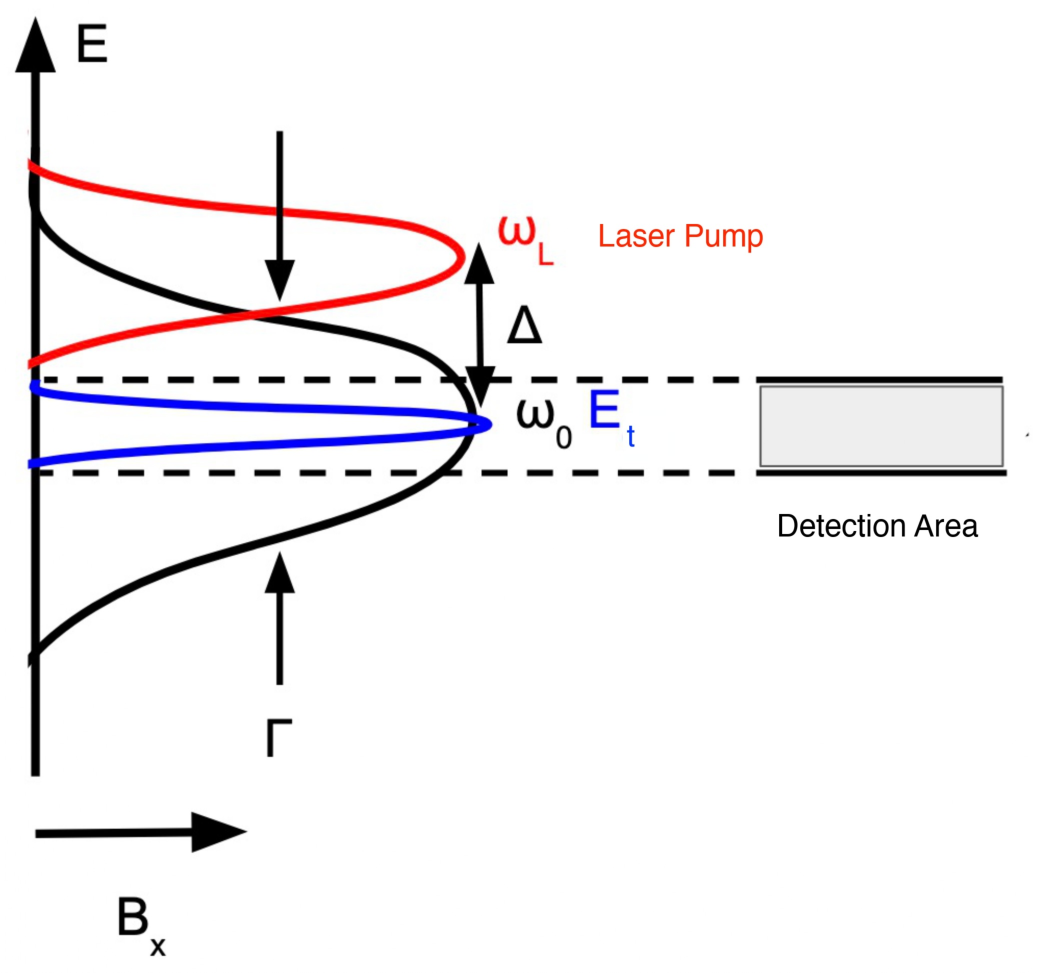
\includegraphics[width=\columnwidth]{scheme_new_v1.pdf}
    \caption{
    Energy scheme of the system.
    The cavity mode of width $\Gamma$ (black) is centered at $\omega_0$ and is
    resonant with the trion transition $E_t$ (blue).
    The pump pulse (red) has the carrier frequency $\omega_L$ and the spectral width
    $\Gamma_L$, and is detuned from the mode by $\Delta$.
    The shaded box marks the spectral window of detection.
    The magnetic field $B_x$ is applied perpendicular to the growth axis.
    }
    \label{fig:scheme}
\end{figure}

Within the rotating wave approximation the Hamiltonian of the system, which
accounts for the coupling to the cavity mode, for the interaction with the
driving laser field and for the interaction with the magnetic field, reads
(hereafter $\hbar = 1$)

\begin{gather}
    \hat{H} = E_t \sum_{\sigma = \uparrow, \downarrow} \hat{d}^{\dag}_{\sigma} \hat{d}_{\sigma}
    + \omega_0 \sum_{\lambda = \pm} \hat{b}^{\dag}_{\lambda} \hat{b}_{\lambda}
    \\ \nonumber
    + g \left( \hat{d}^{\dag}_{\uparrow} \hat{a}_{\uparrow} \hat{b}_{+}
    + \hat{d}^{\dag}_{\downarrow} \hat{a}_{\downarrow} \hat{b}_{-} \right)
    + g^{*} \left( \hat{d}_{\uparrow} \hat{a}^{\dag}_{\uparrow} \hat{b}^{\dag}_{+}
    + \hat{d}_{\downarrow} \hat{a}^{\dag}_{\downarrow} \hat{b}^{\dag}_{-} \right)
    \\ \nonumber
    + \Omega_R(t) \sum_{\sigma = \uparrow, \downarrow}
    \left( \e^{-i \omega_L t} \hat{d}^{\dag}_{\sigma} \hat{a}_{\sigma}
    + \e^{i \omega_L t} \hat{d}_{\sigma} \hat{a}^{\dag}_{\sigma} \right)
    \\ \nonumber
    + \mu_B g_e B_x \left( \hat{a}^{\dag}_{\downarrow} \hat{a}_{\uparrow}
    + \hat{a}^{\dag}_{\uparrow} \hat{a}_{\downarrow} \right)
    + \mu_B g_t B_x \left( \hat{d}^{\dag}_{\downarrow} \hat{d}_{\uparrow}
    + \hat{d}^{\dag}_{\uparrow} \hat{d}_{\downarrow} \right)
    \label{eq:hamiltonian}
\end{gather}
%\begin{gather}
%    \hat{H}_{B} = \mu_B g_e B_x \left( \hat{a}^{\dag}_{\downarrow} \hat{a}_{\uparrow}
%    + \hat{a}^{\dag}_{\uparrow} \hat{a}_{\downarrow} \right)
%    + \mu_B g_t B_x \left( \hat{d}^{\dag}_{\downarrow} \hat{d}_{\uparrow}
%    + \hat{d}^{\dag}_{\uparrow} \hat{d}_{\downarrow} \right)
%    \label{eq:zeeman}
%\end{gather}
where the last two terms describe the Zeeman interaction in the transverse field.
Here $\hat{a}^{\dag}_{\sigma}$ is the creation operator of the resident electron,
where $\sigma = \uparrow, \downarrow$ denotes the spin state $\left| \pm 1/2 \right>$;
$\hat{d}^{\dag}_{\sigma}$ is the creation operator of the negatively charged trion,
where $\sigma$ denotes the heavy hole spin state $\left| \pm 3/2 \right>$;
$\hat{b}^{\dag}_{\pm} = ( \hat{b}^{\dag}_{H} \pm i \hat{b}^{\dag}_{V} ) / \sqrt{2}$
is the creation operator of a cavity photon with circular polarization $\sigma_{\pm}$,
expressed through the linearly polarized modes $H$ and $V$;
$g$ is the effective QD--cavity coupling parameter;
$\mu_B$ is the Bohr magneton, $g_e$ and $g_t$ are the in-plane $g$-factors of the
resident electron and of the trion, respectively.

The optical selection rules fix the spin structure of the light--matter coupling:
a $\sigma_+$ photon converts a resident electron $\left| +1/2 \right>$ into the trion
with the heavy hole $\left| +3/2 \right>$, and a $\sigma_-$ photon converts
$\left| -1/2 \right>$ into $\left| -3/2 \right>$.
Consequently, only the triads $(\hat{a}_{\uparrow}, \hat{d}_{\uparrow}, \hat{b}_{+})$
and $(\hat{a}_{\downarrow}, \hat{d}_{\downarrow}, \hat{b}_{-})$ are coupled, and the
polarization of the emitted photon is rigidly tied to the spin state of the QD.
The transverse field $B_x$, in turn, mixes the two spin branches, which is the
mechanism that correlates the polarizations of the two emitted photons.

%The transformation to the frame rotating with the laser frequency,
%$\hat{d}^{\dag}_{\sigma} \rightarrow \e^{i \omega_L t} \hat{d}^{\dag}_{\sigma}$ and
%$\hat{b}^{\dag}_{\lambda} \rightarrow \e^{i \omega_L t} \hat{b}^{\dag}_{\lambda}$,
%removes the explicit time dependence of Eq.~(\ref{eq:hamiltonian}) and replaces both
%$E_t$ and $\omega_0$ by the single detuning $\Delta$.

To describe the evolution of the system coupled to its environment, the Hamiltonian
dynamics has to be supplemented by the dissipative terms of the Lindblad equation
%% TODO cite Manzano, AIP Advances 10, 025106 (2020)

\begin{gather}
    \partial_t \hat{\rho} = -i \left[ \hat{H}, \hat{\rho} \right]
    + \sum_i \gamma_{i} \left( \hat{V}_i \hat{\rho} \hat{V}_i^{\dag}
    - \frac{1}{2} \left\{ \hat{V}_i^{\dag} \hat{V}_i , \hat{\rho} \right\} \right)
    \equiv \hat{\mathcal{L}} \hat{\rho}
    \label{eq:lindblad}
\end{gather}
where $\{ \cdot , \cdot \}$ is the anticommutator, and $\gamma_i$ and $\hat{V}_i$ are
the rate and the jump operator of the $i$-th channel.
Three dissipation channels are retained.

The first one is the escape of photons from the cavity mode into the environment,
which is the process that delivers the photons to the detector.
Its jump operator and rate are

\begin{gather}
    \hat{V}_{\text{phot}} = \hat{b}_{\pm} , \qquad \gamma_{\text{phot}} = \Gamma
    \label{eq:jump-phot}
\end{gather}
where $\Gamma$ is the width of the cavity mode.

The second channel is the pure dephasing of the optical transition induced by
acoustic phonons, which is responsible for the damping of the Rabi oscillations.
The corresponding jump operator is

\begin{gather}
    \hat{V}_{\text{phon}} = \sum_{\sigma = \uparrow, \downarrow}
    \left( \hat{a}^{\dag}_{\sigma} \hat{a}_{\sigma}
    - \hat{d}^{\dag}_{\sigma} \hat{d}_{\sigma} \right) , \qquad
    \gamma_{\text{phon}} = \alpha \, \Omega_R^2
    \label{eq:jump-phon}
\end{gather}

%The quadratic dependence of the rate on the Rabi frequency corresponds to the
%high-temperature limit $T \gg \Omega_R$ of the exciton--phonon interaction, in which
%the phonon spectral density is sampled at the dressed-state splitting.
%% TODO cite Ramsay PRL 104, 017402 (2010); Ramsay PRL 105, 177402 (2010); Nazir JPCM 28, 103002 (2016)

The third channel is the dephasing of the resident electron spin.
It is described by the operator

%\begin{gather}
%    \hat{V}_{\text{spin i}} = \hat{a}^{\dag}_{\uparrow} \hat{a}_{\uparrow}
%    - \hat{a}^{\dag}_{\downarrow} \hat{a}_{\downarrow}
%    + \hat{d}^{\dag}_{\uparrow} \hat{d}_{\uparrow}
%    - \hat{d}^{\dag}_{\downarrow} \hat{d}_{\downarrow} , \qquad
%    \gamma_{\text{spin}} = \dots
%    \label{eq:jump-spin}
%\end{gather}

\begin{gather}
    \hat{V}_{\text{spin} \, i} =
\begin{pmatrix}
    \hat{a}^{\dag}_{\uparrow} & \hat{a}^{\dag}_{\downarrow}
\end{pmatrix}
    \hat{\sigma}_i
\begin{pmatrix}
    \hat{a}_{\uparrow} \\
    \hat{a}_{\downarrow}
\end{pmatrix} +
\begin{pmatrix}
    \hat{d}^{\dag}_{\uparrow} & \hat{d}^{\dag}_{\downarrow}
\end{pmatrix}
    \hat{\sigma}_i
\begin{pmatrix}
    \hat{d}_{\uparrow} \\
    \hat{d}_{\downarrow}
\end{pmatrix}
    \label{eq:jump-spin}
\end{gather}

where $\hat{\sigma}_i$ with $i = x, y, z$ are the Pauli matrices acting in the spin
space of the resident electron and of the trion.
Since the magnetic field is directed along $x$, the operators
$\hat{V}_{\text{spin} \, y}$ and $\hat{V}_{\text{spin} \, z}$ relax the transverse
spin component, whereas $\hat{V}_{\text{spin} \, x}$ adds a pure dephasing of the
longitudinal ones.
The three rates are therefore expressed through the longitudinal and transverse spin
relaxation times $T_1$ and $T_2$ as

\begin{gather}
    \gamma_{\text{spin} \, x} = \frac{1}{T_1} , \qquad
    \gamma_{\text{spin} \, y} = \gamma_{\text{spin} \, z} = \frac{1}{T_2}
    \label{eq:spin-rates}
\end{gather}

This channel destroys the coherence between the two spin branches and therefore
directly degrades the polarization entanglement of the emitted photon pair.

Equation~(\ref{eq:lindblad}) is solved with the initial condition set by the state
of the system before the arrival of the pump pulse, when the cavity mode is empty
and the QD hosts only the resident electron.
In the transverse magnetic field the eigenstates of the electron spin are the
symmetric and antisymmetric superpositions
$( \left| \uparrow \right> \pm \left| \downarrow \right> ) / \sqrt{2}$
split by the energy $2 \mu_B g_e B_x$, and their populations follow the
Boltzmann distribution at the lattice temperature $T$.
The initial density matrix therefore reads

\begin{gather}
    \hat{\rho}_0 =
    \frac{f(B_x)}{2}
    \left(\hat{a}^{\dag}_{\uparrow} + \hat{a}^{\dag}_{\downarrow} \right)
    \left| 0 \right> \left< 0 \right|
    \left(\hat{a}_{\uparrow} + \hat{a}_{\downarrow} \right)
    \label{eq:rho0}
    \\ \nonumber
    + \frac{f(-B_x)}{2}
    \left(\hat{a}^{\dag}_{\uparrow} - \hat{a}^{\dag}_{\downarrow} \right)
    \left| 0 \right> \left< 0 \right|
    \left(\hat{a}_{\uparrow} - \hat{a}_{\downarrow} \right)
\end{gather}
where $f(B_x) = \e^{\mu_B g_e B_x / T}/ \left( \e^{\mu_B g_e B_x / T} + \e^{-\mu_B g_e B_x / T}  \right)$
and the temperature is measured in energy units.

The quantities measured in the experiment are the polarizations of the photons that
reach the detector, so the observables are given by the projections of the full
density matrix onto the sectors with a fixed number of emitted photons.
Following Ref.~\cite{Krainov}, these sectors are conveniently expressed through the
propagator $\e^{\hat{\mathcal{L}} t}$ of the Lindbladian,

\begin{gather}
    \hat{\rho}(t) = \e^{\hat{\mathcal{L}} t} \hat{\rho}_0
    \label{eq:propagator}
\end{gather}

The one- and two-photon density matrices in the basis of the circular polarizations
$\lambda = \pm$ then read

\begin{gather}
    \left( \hat{\rho}_1 \right)_{\lambda \lambda'} =
    \Gamma \int dt_1 \, \text{Tr}
    \left( \hat{b}_{\lambda} \, \hat{\rho}(t_1) \, \hat{b}^{\dag}_{\lambda'} \right)
    \label{eq:rho1}
\end{gather}

\begin{gather}
    \left( \hat{\rho}_2 \right)_{\lambda_1 \lambda_2 , \lambda_1' \lambda_2'} =
    \Gamma^2 \int dt_1 dt_2 \, \text{Tr}
    \Big( \hat{b}_{\lambda_2} \, \e^{\hat{\mathcal{L}} (t_2 - t_1)}
    \\ \nonumber
    \times \left[ \hat{b}_{\lambda_1} \, \hat{\rho}(t_1) \, \hat{b}^{\dag}_{\lambda_1'} \right]
    \hat{b}^{\dag}_{\lambda_2'} \Big)
    \label{eq:rho2}
\end{gather}
where $\text{Tr}$ denotes the trace over all states except the photon states with
$n = 0, 1, 2$.
The probabilities of the one- and two-photon emission are the traces of these
matrices,

\begin{gather}
    P_1 = \text{Tr} \, \hat{\rho}_1 , \qquad P_2 = \text{Tr} \, \hat{\rho}_2
    \label{eq:p1p2}
\end{gather}

As shown in Ref.~\cite{Krainov}, $\hat{\rho}_2$ contains two contributions of
different nature: the resonant scattering of the laser photons, in which the whole
dynamics stays coherent, and the re-excitation, in which the first photon actually
leaves the cavity during the pulse and the remaining part of the pulse drives the QD
again.

\begin{figure*}
    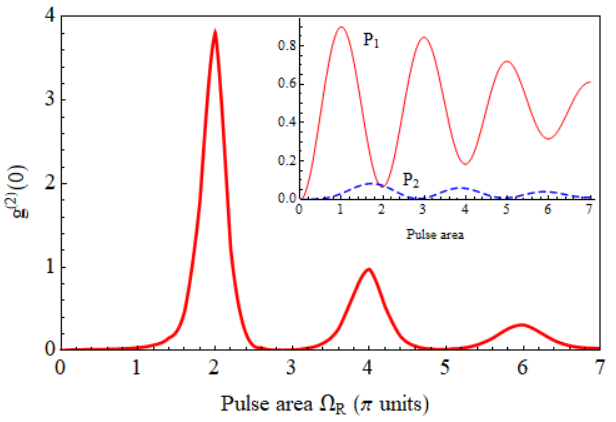
\includegraphics[width=1\columnwidth]{g2_p1_p2_v2.png}
    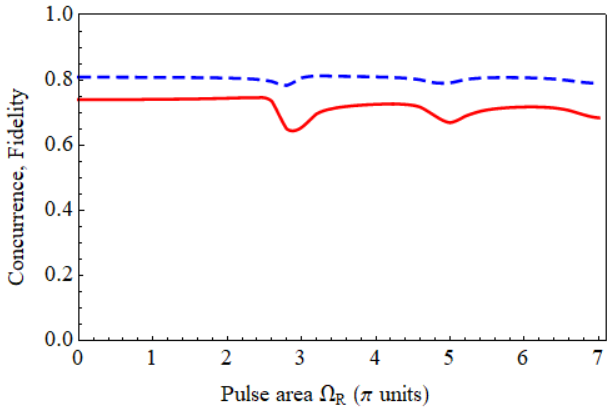
\includegraphics[width=1\columnwidth]{conc_fidel_v2.png}
    \caption{
    (Left) Second-order correlation function at zero delay, $g^{(2)}(0)$, as a function of the pump pulse area. Inset: Probabilities of the one-photon, $P_1$ (solid), and two-photon, $P_2$ (dashed), emission as functions of the pump pulse area.
    (Right) Concurrence (solid) of the emitted two-photon polarization state and fidelity (dashed) to the Bell state $\left| \Phi^+ \right>$ as a function of the
    pump pulse area.
    }
    \label{fig:results}
\end{figure*}

In our case the pulse is short, $\Gamma \tau \sim 1$, and in this regime the resonant
scattering dominates \cite{Krainov}.
Neglecting the escape of the photon from the mode during the pulse and the
phonon-induced dephasing, the dynamics of this contribution is described by the
following scheme

\begin{gather}
    \hat{a}^{\dag}_{\uparrow} \left| 0 \right> + \hat{a}^{\dag}_{\downarrow} \left| 0 \right>
    \; \xrightarrow{\ \Omega_R \ } \;
    \hat{d}^{\dag}_{\uparrow} \left| 0 \right> + \hat{d}^{\dag}_{\downarrow} \left| 0 \right>
    \label{eq:scheme}
    \\ \nonumber
    \xrightarrow{\ 2\pi \ } \;
    \hat{b}^{\dag}_{+L} \hat{d}^{\dag}_{\uparrow} \left| 0 \right>
    + \hat{b}^{\dag}_{-L} \hat{d}^{\dag}_{\downarrow} \left| 0 \right>
    \\ \nonumber
    \longrightarrow \;
    \hat{b}^{\dag}_{+L} \hat{b}^{\dag}_{+t} \hat{a}^{\dag}_{\uparrow} \left| 0 \right>
    + \hat{b}^{\dag}_{-L} \hat{b}^{\dag}_{-t} \hat{a}^{\dag}_{\downarrow} \left| 0 \right>
    \\ \nonumber
    \xrightarrow{\ \text{spin relax} \ } \;
    \left( \hat{b}^{\dag}_{+L} \hat{b}^{\dag}_{+t}
    + \hat{b}^{\dag}_{-L} \hat{b}^{\dag}_{-t} \right)
    \left( \hat{a}^{\dag}_{\uparrow} + \hat{a}^{\dag}_{\downarrow} \right) \left| 0 \right>
\end{gather}
where $\hat{b}^{\dag}_{\lambda L}$ creates the resonantly scattered laser photon and
$\hat{b}^{\dag}_{\lambda t}$ the photon emitted upon the trion recombination.
The pulse first drives the resident electron into the trion, then a laser photon is
resonantly scattered into the mode, and finally the trion recombines, returning the
QD to its ground state.

The two-photon density matrix therefore carries, besides the two photon
polarizations, a third index, the spin of the resident electron.
The selection rules tie all three of them together: each pair of co-polarized photons
is emitted together with a definite spin projection left in the QD, so that the
photons remain entangled with the electron.
The spin relaxation towards the in-plane thermal state, the last step of
Eq.~(\ref{eq:scheme}), is what breaks this link.
It decouples the photonic degrees of freedom from the electronic ones at the price of
a slightly reduced entanglement of the pair, since the spin coherence that survives
the relaxation is limited by the thermal factor
$\tanh \left( \mu_B g_e B_x / T \right)$.

Written as a density matrix with the thermal weights taken into account, the last
line of Eq.~(\ref{eq:scheme}) gives, to first order in $g \tau$ and in the basis
$\left| + + \right>$, $\left| + - \right>$, $\left| - + \right>$,
$\left| - - \right>$,

\begin{gather}
    \hat{\rho}_2^{(2\pi)} \approx \left( g \tau \right)^2
    \left( \frac{\Omega_R^2}{\Omega_R^2 + \Delta^2} \right)^2
    \begin{pmatrix}
        1 & 0 & 0 & \eta^2 \\
        0 & 0 & 0 & 0 \\
        0 & 0 & 0 & 0 \\
        \eta^2 & 0 & 0 & 1
    \end{pmatrix}
    \label{eq:rho2-analytic}
\end{gather}
where $\eta = \tanh \left( \mu_B g_e B_x / T \right)$.
Only the co-polarized states $\left| + + \right>$ and $\left| - - \right>$ are
populated, and the entire dependence on the magnetic field and on the temperature
enters through the coherence $\eta^2$.
The square appears because the spin coherence is picked up twice, once through the
initial state (\ref{eq:rho0}) and once through the spin left behind after the
emission.
The factor $\Omega_R^2 / ( \Omega_R^2 + \Delta^2 )$ shows how the detuning influences
the two-photon yield.

Equation~(\ref{eq:rho2-analytic}) is a mixture of two Bell states with thermal
weights,

\begin{gather}
    \hat{\rho}_2^{(2\pi)} \propto \frac{1 + \eta^2}{2}
    \left| \Phi^+ \right> \left< \Phi^+ \right|
    + \frac{1 - \eta^2}{2}
    \left| \Phi^- \right> \left< \Phi^- \right|
    \label{eq:bell-mixture}
\end{gather}

where $\left| \Phi^{\pm} \right> = ( \left| + + \right> \pm
\left| - - \right> ) / \sqrt{2}$.
In the limit of a strong spin polarization, $\mu_B g_e B_x \gg T$,
$\eta \rightarrow 1$ and only the maximally entangled $\left| \Phi^+ \right>$
survives, whereas for $\mu_B g_e B_x \ll T$ the two Bell states enter with equal
weights and the pair is no longer entangled.

The quality of the generated state is characterized by two standard measures.
The first one is the fidelity to the target Bell state,

\begin{gather}
    F = \left< \Phi^+ \right| \hat{\rho}_2 \left| \Phi^+ \right>
    \label{eq:fidelity}
\end{gather}

which exceeds $1/2$ only for entangled states and therefore already serves as an
entanglement witness.
The second one is the concurrence, which quantifies the entanglement itself,
%% TODO cite Wootters, PRL 80, 2245 (1998)

\begin{gather}
    C = \max \left( 0 , \, \lambda_1 - \lambda_2 - \lambda_3 - \lambda_4 \right)
    \label{eq:concurrence}
\end{gather}

where $\lambda_1 \geq \lambda_2 \geq \lambda_3 \geq \lambda_4$ are
the eigenvalues of the matrix $\sqrt{\sqrt{\hat{\rho}_2} \hat{\tilde{\rho}}_2 \sqrt{\hat{\rho}_2} }$, and
$\hat{\tilde{\rho}}_2 = \left( \hat{\sigma}_y \otimes \hat{\sigma}_y \right)
\hat{\rho}_2^{*} \left( \hat{\sigma}_y \otimes \hat{\sigma}_y \right)$ is the spin
flipped density matrix, the complex conjugation being taken in the polarization
basis.
The concurrence vanishes for separable states and reaches unity for a maximally
entangled one.

All the results presented below are obtained by a numerical solution of
Eq.~(\ref{eq:lindblad}) with the following set of parameters:
the cavity mode width $\Gamma = 50\,\mu\text{eV}$, the QD--cavity coupling
$g = 25\,\mu\text{eV}$, the detuning $\Delta = 50\,\mu\text{eV}$, the pulse duration
$\tau = 13\,\text{ps}$, the phonon coupling constant $\alpha = 0.15\,\text{ps}$, the
transverse magnetic field $B_x = 5\,\text{T}$ and the lattice temperature
$T = 1\,\text{K}$.
The pulse area $\theta = \int \Omega_R(t) \, dt$ is varied by changing the pump
power at a fixed pulse duration, and is measured below in units of $\pi$.
%Equivalently, in the basis
%$\{ \hat{a}^{\dag}_{\uparrow} \left| 0 \right> ,
%\hat{a}^{\dag}_{\downarrow} \left| 0 \right> \}$ the populations of the two spin
%projections are equal and the off-diagonal element of $\hat{\rho}_0$ equals
%$\tanh \left( \mu_B g_e B_x / T \right) / 2$.
%The single parameter $\mu_B g_e B_x / T$ thus controls the degree of the initial
%spin coherence.
%For $\mu_B g_e B_x \gg T$ the electron is fully polarized along the field and the
%system starts from a pure state, whereas for $\mu_B g_e B_x \ll T$ the initial
%state is a fully incoherent mixture.
%Since the polarization correlations of the emitted pair are inherited from the
%coherence between the two spin branches, this ratio directly limits the entanglement
%of the outgoing two-photon state.



The emission probabilities are shown in the inset of Fig.~\ref{fig:results}.
The one-photon probability $P_1$ exhibits damped Rabi oscillations with maxima at odd
and minima at even multiples of $\pi$, the damping being caused by the
phonon-induced dephasing.
The two-photon probability $P_2$ oscillates in antiphase and remains an order of
magnitude smaller, reaching its maxima close to even pulse areas.

This antiphase behaviour is directly reflected in the second-order correlation
function, Fig.~\ref{fig:results}.
At odd pulse areas $g^{(2)}(0)$ nearly vanishes, so that the source emits single
photons, whereas at even ones it displays pronounced bunching peaks, the largest
reaching $g^{(2)}(0) \approx 3.8$ at $\theta = 2\pi$.

The polarization state of the emitted pair is characterized in
Fig.~\ref{fig:results}.
Both the concurrence and the fidelity to the Bell state
$\left| \Phi^+ \right>$ are only weakly sensitive to the pump power, staying close
to $0.7$ and $0.8$, respectively, over the whole range of pulse areas, with
shallow minima near the odd ones.
The fidelity exceeding $1/2$ confirms that the emitted pair is entangled for any
excitation power.


\end{document}